
\documentclass[9pt]{beamer}
%\makeatletter
%\def\beamer@calltheme#1#2#3{%
%	\def\beamer@themelist{#2}
%	\@for\beamer@themename:=\beamer@themelist\do
%	{\usepackage[{#1}]{\beamer@themelocation/#3\beamer@themename}}}
%
%\def\usefolder#1{
%	\def\beamer@themelocation{#1}
%}
%\def\beamer@themelocation{}

%\usefolder{../config}

\usetheme[
block=fill,
titleformat=regular,
progressbar=frametitle
]{metropolis}
%\metroset[everytitleformat=regular] % regular, lowercase, uppercase ]
%\metroset[inner/block=fill]

%\setbeameroption{show notes} 
\usepackage{booktabs}
\usepackage[scale=2]{ccicons}

\usepackage{pgfplots}
\usepgfplotslibrary{dateplot}


%\ Hrvatski znakovi
\usepackage[utf8]{inputenc}
\usepackage[T1]{fontenc}
\usepackage[croatian]{babel}
\usepackage{todonotes}
\usepackage{amsmath}
\usepackage{amsfonts}
\selectlanguage{croatian} % american ngerman
\usepackage{todonotes}

% Koristenje Latin modern fonta
% Bez toga na nekim racunalima baca
% err: Font <taj i taj> at <mala velicina, npr4.0pt> not loadable: Metric (TFM) file not found. \end{frame}
\usepackage{lmodern}


\definecolor{RoyalBlue}{cmyk}{1, 0.50, 0, 0}
%\usepackage{natbib}
%\usepackage{bibentry}
\usepackage{scrextend}
\usepackage{hyperref}
%\usepackage[pdfa=true]{hyperref}
\hypersetup{%
    %draft, % = no hyperlinking at all (useful in b/w printouts)
    %colorlinks=true, 
    linktocpage=true, pdfstartpage=3, pdfstartview=FitV,%
    % uncomment the following line if you want to have black links (e.g., for printing)
    %colorlinks=false, linktocpage=false, pdfborder={0 0 0}, pdfstartpage=3, pdfstartview=FitV,% 
    breaklinks=true, pdfpagemode=UseNone, pageanchor=true, pdfpagemode=UseOutlines,%
    plainpages=false, bookmarksnumbered, bookmarksopen=true, bookmarksopenlevel=1,%
    hypertexnames=true, pdfhighlight=/O,%nesting=true,%frenchlinks,%
    %urlcolor=webbrown, linkcolor=RoyalBlue, citecolor=webgreen, %pagecolor=RoyalBlue,%
    %urlcolor=Blue, linkcolor=Blue, citecolor=Red, %pagecolor=Black,%
    %pdftitle={\myTitle},%
    %pdfauthor={\textcopyright\ \myName, \myUni, \myFaculty},%
    pdfsubject={},%
    pdfkeywords={},%
    pdfcreator={pdfLaTeX},%
    pdfproducer={LaTeX with hyperref and classicthesis}, %
    unicode = true 
} 

%\usepackage[pdftex]{graphicx}
% declare the path(s) where your graphic files are
\graphicspath{{./}{./figures/}}


\newcommand{\executeiffilenewer}[3]{%
	\ifnum\pdfstrcmp{\pdffilemoddate{#1}}%
	{\pdffilemoddate{#2}}>0%
	{\immediate\write18{#3}}\fi%
}
\newcommand{\includesvg}[1]{%
	\executeiffilenewer{#1.svg}{#1.pdf}%
	{inkscape -z -C --file=#1.svg %
		--export-pdf=#1.pdf --export-latex}%
	\input{#1.pdf_tex}%
}


% http://tex.stackexchange.com/questions/83882/how-to-highlight-python-syntax-in-latex-listings-lstinputlistings-command

\usepackage{listings}
\usepackage{color}
\usepackage[semibold]{sourcecodepro}

% Default fixed font does not support bold face
\DeclareFixedFont{\ttb}{T1}{txtt}{bx}{n}{12} % for bold
\DeclareFixedFont{\ttm}{T1}{txtt}{m}{n}{12}  % for normal
% Custom colors
\definecolor{deepblue}{rgb}{0,0,0.5}
\definecolor{deepred}{rgb}{0.6,0,0}
\definecolor{deepgreen}{rgb}{0,0.5,0}


% Python style for highlighting
\newcommand\pythonstyle{\lstset{
		language=Python,
		basicstyle=\small\ttfamily,
		otherkeywords={self},             % Add keywords here
		keywordstyle=\small\ttfamily\color{deepblue},
		emph={MyClass,__init__},          % Custom highlighting
		emphstyle=\small\ttfamily\color{deepred},    % Custom highlighting style
		stringstyle=\color{deepgreen},
		frame=tb,                         % Any extra options here
		showstringspaces=false            % 
	}}
	
	
	% Python environment
	\lstnewenvironment{python}[1][]
	{
		\pythonstyle
		\lstset{#1}
	}
	{}
	
	% Python for external files
	\newcommand\pythonexternal[2][]{{
			\pythonstyle
			\lstinputlisting[#1]{#2}}}
	
	% Python for inline
	\newcommand\pythoninline[1]{{\pythonstyle\lstinline!#1!}}
%\documentclass[ucs]{beamer}
%\usetheme[menuwidth={0.3\paperwidth}]{erlangen}
%\setbeamercovered{transparent=20} 

\usepackage{amsmath,amsfonts,amsthm,amssymb}
\usepackage{setspace}
\usepackage{Tabbing}
\usepackage{fancyhdr}
\usepackage{lastpage}
\usepackage{extramarks}
\usepackage{chngpage}
\usepackage{soul,color}
\usepackage{graphicx,float,wrapfig}
\usepackage{xcolor}
\usepackage[normalem]{ulem}
\usepackage{mathtools}
\usepackage{cancel}

\definecolor{erlangenlyellow}{RGB}{123, 25, 121}
%\usepackage[utf8x]{inputenc}
%\usepackage{default}
%\usepackage[T1]{fontenc}

\usepackage{verbatim}
\usepackage{listings}
\usepackage{algorithm2e}


\usepackage{subcaption}
\usepackage{lmodern}

\title{Ray tracing}

\subtitle{Podnaslov}
\institute{Računalna grafika}

% Delete this, if you do not want the table of contents to pop up at
% the beginning of each subsection:
%\AtBeginSubsection[]
%{
%  \begin{frame}<beamer>{Outline}
%    \tableofcontents[currentsection,currentsubsection]
%  \end{frame}
%}
%
%\AtBeginSection[]
%{
%  \begin{frame}<beamer>{Outline}
%    \tableofcontents[currentsection]
%  \end{frame}
%}

\begin{document}
\begin{frame}
 \titlepage
\end{frame}

\begin{frame}{Sadržaj}
  \tableofcontents
  % You might wish to add the option [pausesections]
\end{frame}

%
%\begin{frame}{Render jednadžba}
%	\begin{align*}
%	L_o(X, \hat{\omega}_o) = L_e(X, \hat{\omega}_e) +
%	 \int_{S^2}  L_i(X, \hat{\omega}_i) f_X(\hat{\omega}_i), \hat{\omega}_o)) \left|\hat{\omega}_i\cdot \hat{n}\right| 
%	 \mathrm{d} \hat{\omega}_i
%	\end{align*}
%	\begin{itemize}
%		\item $X$: točka u sceni
%		\item $\hat{\omega}_o$: izlazni smjer(\textit{outgoing dir}), smjer prema očištu
%		\item $\hat{\omega}_i$: dolazni, ulazni smjer(\textit{incoming dir}), smjer svjetla na točku $X$ 
%    	\item $\hat{n}$: normala površine
%		\item $S^2$: svi dolazni, ulazni smjerovi(\textit{incoming directions})
%	\end{itemize}
%\end{frame}
%
%\begin{frame}{Render jednadžba}
%	\begin{align*}
%	L_o(X, \hat{\omega}_o) = L_e(X, \hat{\omega}_e) +
%	\int_{S^2}  L_i(X, \hat{\omega}_i) f_X(\hat{\omega}_i), \hat{\omega}_o)) \left|\hat{\omega}_i\cdot \hat{n}\right| 
%	\mathrm{d} \hat{\omega}_i
%	\end{align*}
%	\begin{itemize}
%		\item $L_o(X, \hat{\omega}_o)$: Izlazno svjetlo - Kakav je rezultirajući intenzitet svjetla za zadanu točku i smjer?
%		\item $L_e(X, \hat{\omega}_e)$: Emitirano svjetlo - Kakav je intenzitet svjetla koji emitira zadana točka za zadani smjer? - Recimo izvor svjetla
%		\item $L_i(X, \hat{\omega}_i)$: Dolazno, ulazno svjetlo - za zadanu točku koji intenzitet svjetla vidim za zadani smjer?
%		\item $f_X(\hat{\omega}_i), \hat{\omega}_o))$: Materijal - za zadani ulazni i izlazni smjer, koji intenzitet svjetla ide u izlaznom smjeru?
%		\item $\left|\hat{\omega}_i\cdot \hat{n}\right|$: Lambert - geometrijski izraz, recimo, difuzni 
%	\end{itemize}
%\end{frame}
%
%\begin{frame}{Render jednadžba}
%	\begin{align*}
%	L_o(X, \hat{\omega}_o) = L_e(X, \hat{\omega}_e) +
%	\int_{S^2}  L_i(X, \hat{\omega}_i) f_X(\hat{\omega}_i), \hat{\omega}_o)) \left|\hat{\omega}_i\cdot \hat{n}\right| 
%	\mathrm{d} \hat{\omega}_i
%	\end{align*}
%	\begin{itemize}
%		\item $S^2$: svi dolazni, ulazni smjerovi(\textit{incoming directions})
%		\item $\mathrm{d} \hat{\omega}_i$
%	\end{itemize}
%Pure Path tracing: zbrojimo sva svjetla iz svih smjerova
%\end{frame}



\section{Sjene}

\begin{frame}{Sjene}
\begin{center}
	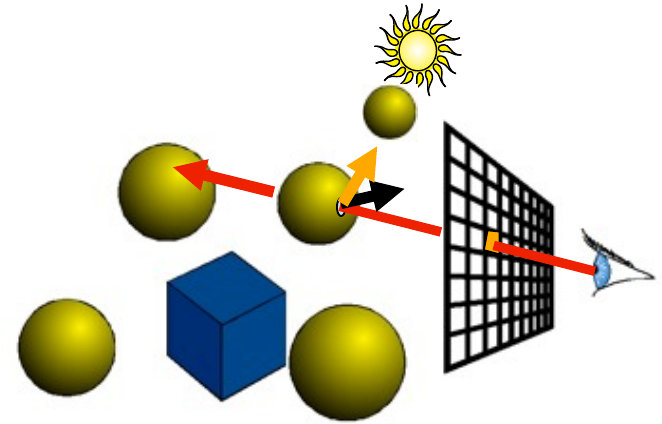
\includegraphics[width=8cm]{slike/sjene_01.png}
\end{center}

\end{frame}

\begin{frame}{Sjene, kostur algoritma}
\begin{algorithm*}[H]
%\KwResult{Write here the result }
color = ka*hit.material().kd()\;
\For{ za svaki izvor svjetla}
{
	Ray ray2(hitPoint, directionToLight)\;
	ambient = ka\;
	Hit hit2(distanceToLight)\;
	\For{ za svaki objekt}
	{
		object.intersect(ray2, hit2)\;
		%diffuseColor = object.intersect(ray2, hit2)\;
		\If{hit2->getT() == distanceToLight}
		{
			color += hit.getMaterial().shade(ray, hit, directionToLight, lightColor)\;
		}
	}
	
}
return color\;
%\caption{How to write algorithms}
\end{algorithm*}
\end{frame}

\begin{frame}{Sjene, contd.}
\begin{center}
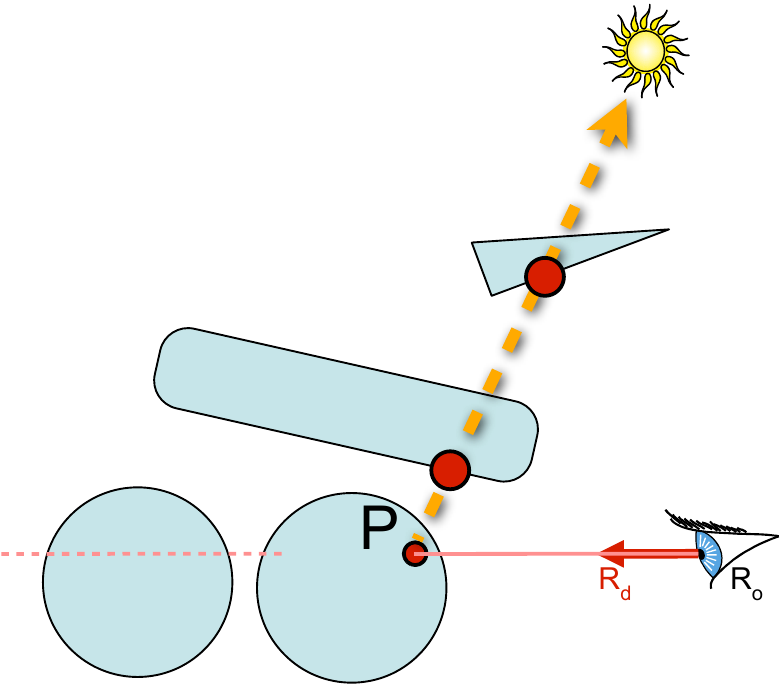
\includegraphics[width=4cm]{slike/sjene_02.png}
\end{center}
U čemu se razlikuju \textit{shadow} zrake u odnosu na \textit{eye} zrake?\\
Nije potrebno naći najbliži objekt, dovoljno je da je samo jedan između zrake i izvora svjetla 
\end{frame}

\section{Refleksija}
\begin{frame}{Refleksija}

\begin{center}
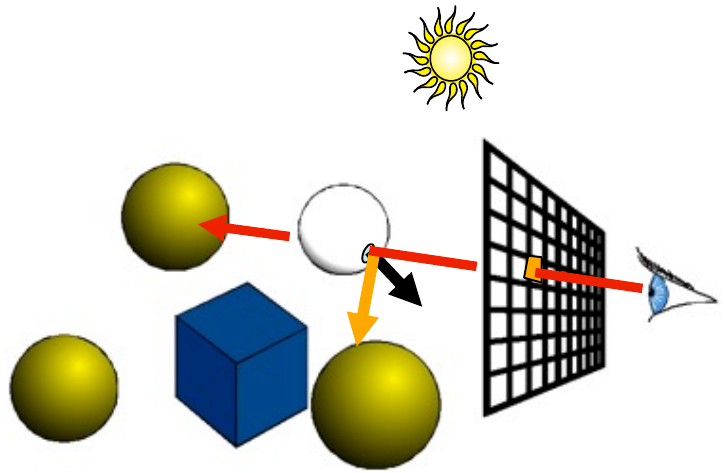
\includegraphics[width=5cm]{slike/refleksija_01.png}
\end{center}
\begin{itemize}
\item Odaslati zraku simetrično na normalu
\item pomnožiti sa zrcalnom komponentom $k_s$, ili nešto slično tome
\end{itemize}
\end{frame}

\begin{frame}{Refleksija, kako izračunati zrcalnu zraku}

\begin{center}
	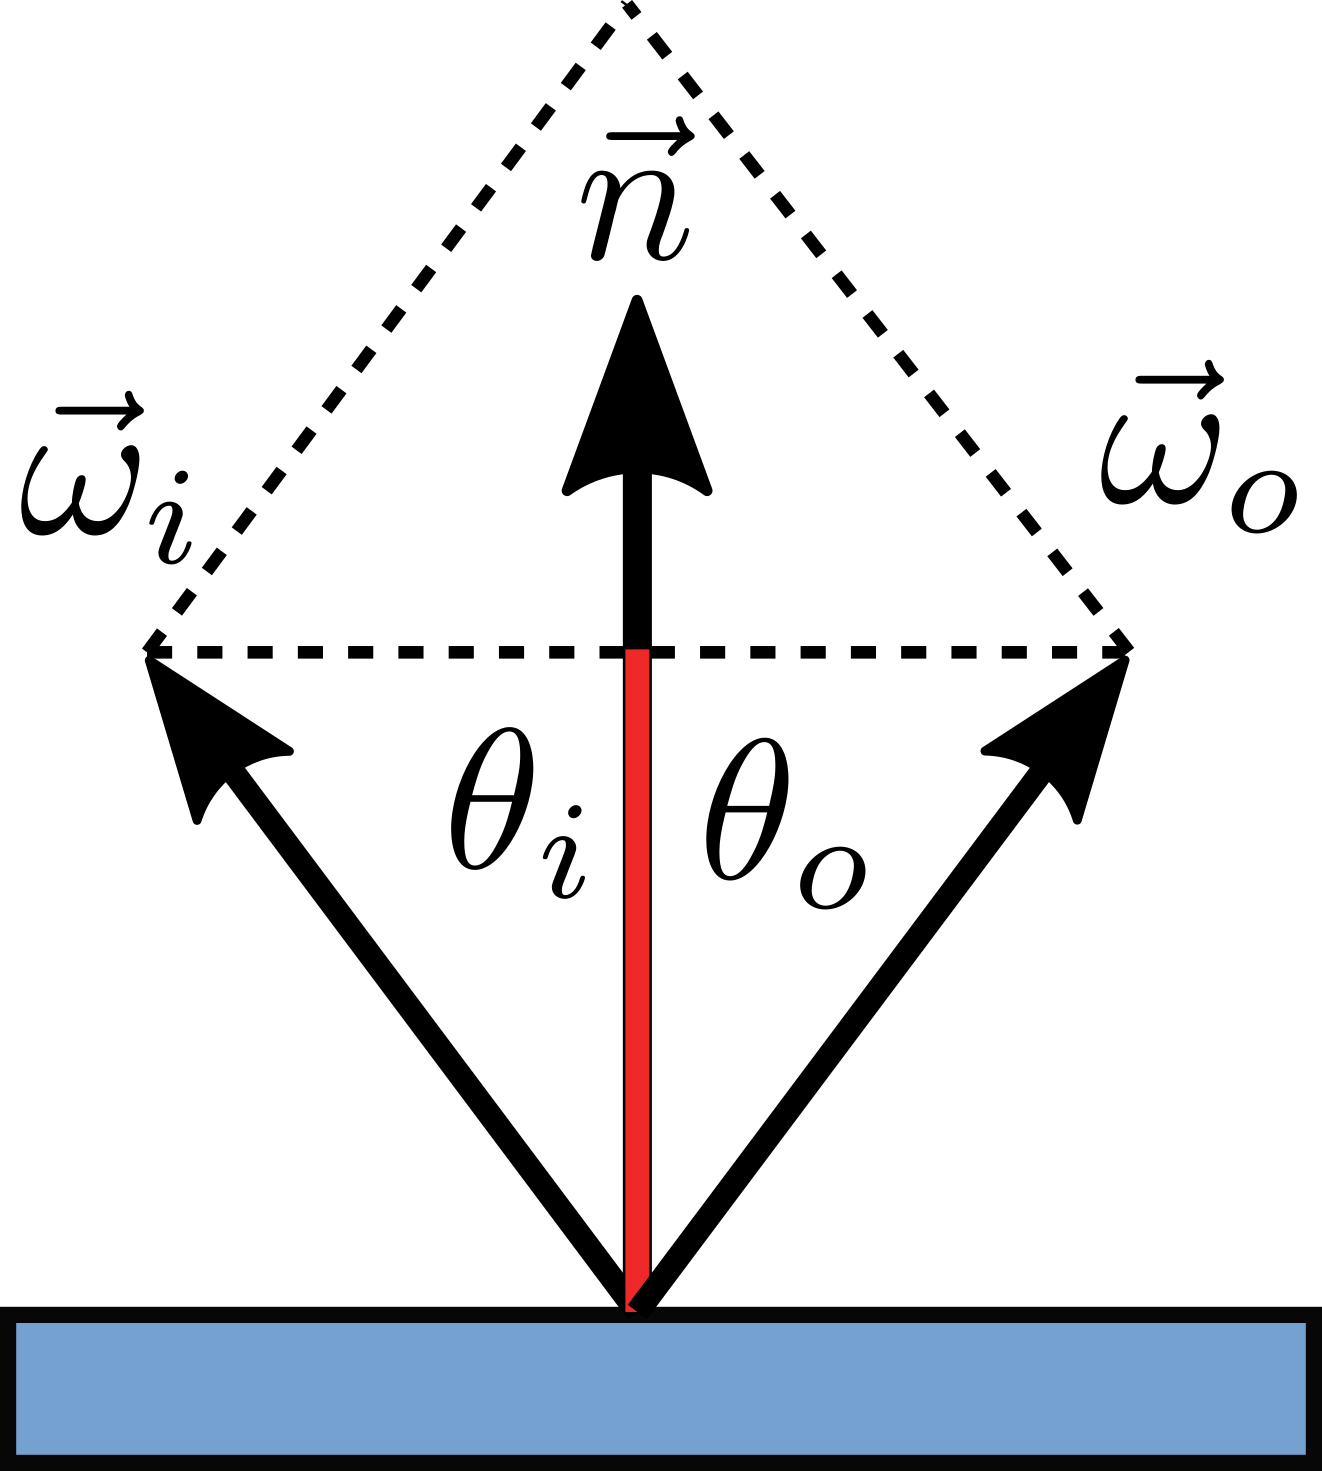
\includegraphics[width=3cm]{slike/refleksija.png}
\end{center}
\begin{align*}
	\theta= \theta_i = \theta_t
\end{align*}
\begin{align*}
\vec{\omega}_i + \vec{\omega}_o & = 2 \cos \theta \vec{n} = 2(\vec{\omega}_i \cdot \vec{n})\vec{n} \\
 \vec{\omega}_o & = -\vec{\omega}_i + 2(\vec{\omega}_i \cdot \vec{n})\vec{n}
\end{align*}
\end{frame}

\section{Difuzni i refleksivni materijali}
\begin{frame}{Difuzni materijal}
	\begin{center}
		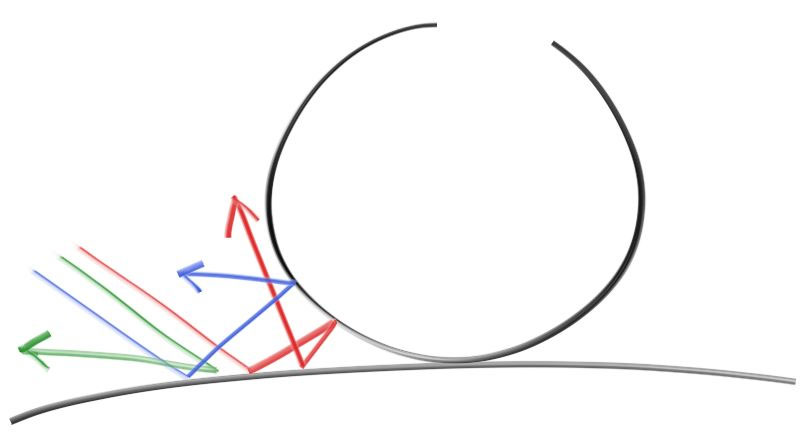
\includegraphics[width=6cm]{slike/fig-1.08-light-bounce.jpg}
	\end{center}

\end{frame}

\begin{frame}{Difuzni materijal}
	\begin{columns}
		\begin{column}{0.3\textwidth}
			\begin{center}
				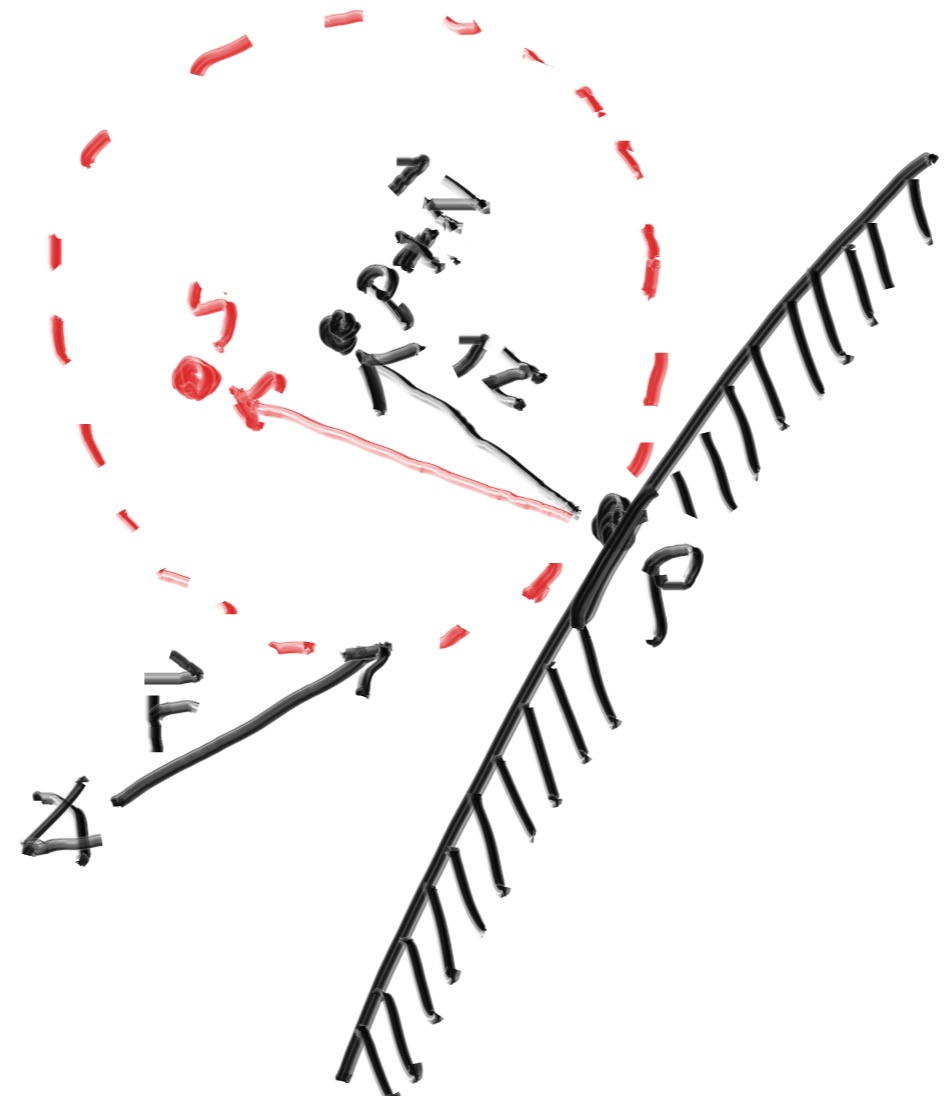
\includegraphics[width=4cm]{slike/fig-1.09-rand-vec.jpg}
			\end{center}
		\end{column}
	\begin{column}{0.7\textwidth}
		\begin{enumerate}
			\item Središta sfera: $\mathbf{P} + \mathbf{n}$ i $\mathbf{P} - \mathbf{n}$
			\item $\mathbf{P} - \mathbf{n}$ unutar, $\mathbf{P} + \mathbf{n}$ izvan
			\item Odabrati nasumičnu točku $\mathbf{S}$
			\item Definirati zraku koja prolazi kroz točke $\mathbf{P}$ i $\mathbf{S}$
			\item Odrediti koeficijent kojim se apsorbira svjetlost (intenzitet, nota bene)  :recimo $1/2$, $2/5$ $\ldots$
			\item Provjeriti siječe li se ta zraka s nekim objektom
			\item go to 3
			\item Funkcija je rekurzivna, obično se definira broj odbijanja (dubina): npr. $20, 30, 50, 100, \ldots$
		\end{enumerate}
	\end{column}
	\end{columns}
\end{frame}

\begin{frame}{Difuzni materijal}
	\begin{columns}
		\begin{column}{0.3\textwidth}
			\begin{center}
				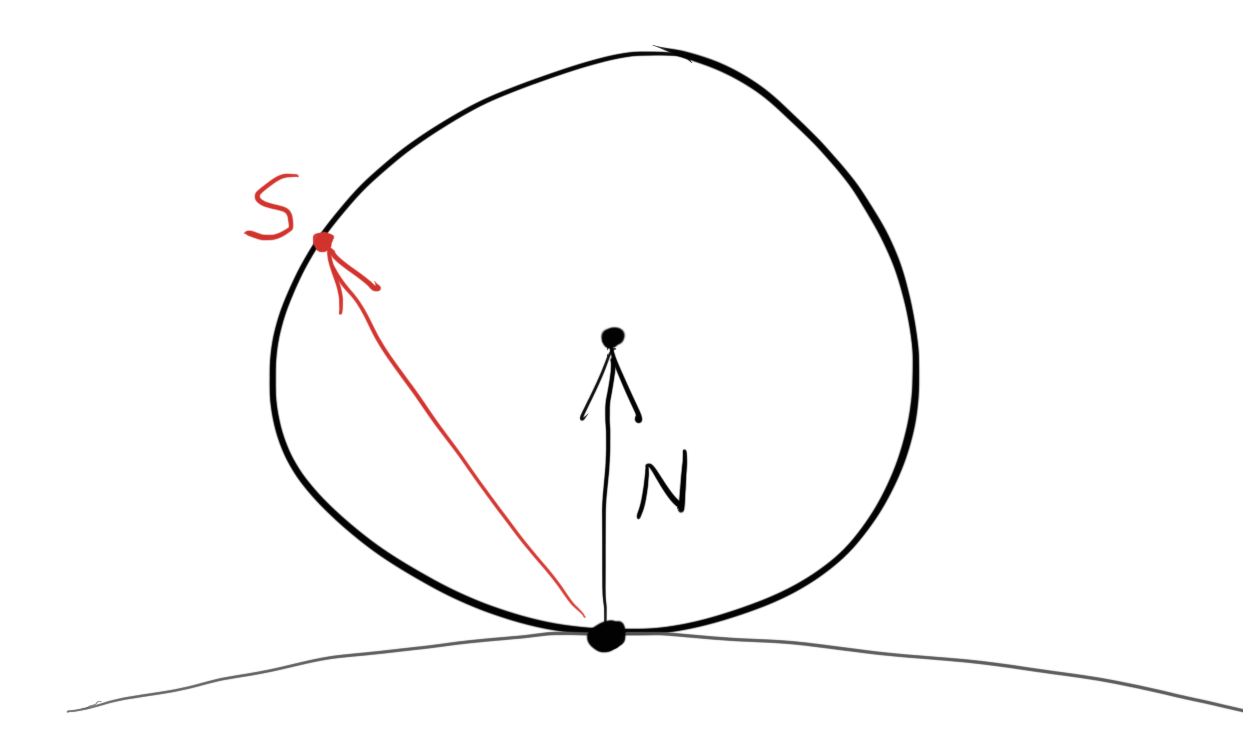
\includegraphics[width=4cm]{slike/fig-1.10-rand-unitvec.png}
			\end{center}
		\end{column}
		\begin{column}{0.7\textwidth}
			\begin{enumerate}
				\item Središta sfera: $\mathbf{P} + \mathbf{n}$ i $\mathbf{P} - \mathbf{n}$
				\item $\mathbf{P} - \mathbf{n}$ unutar, $\mathbf{P} + \mathbf{n}$ izvan
				\item \alert{Bolje: Odabrati nasumičnu točku $\mathbf{S}$ \textbf{na površini kugle} }
				\item Definirati zraku koja prolazi kroz točke $\mathbf{P}$ i $\mathbf{S}$
				\item Odrediti koeficijent kojim se apsorbira svjetlost (intenzitet, nota bene)  :recimo $1/2$, $2/5$ $\ldots$
				\item Provjeriti siječe li se ta zraka s nekim objektom
				\item go to 3
				\item Funkcija je rekurzivna, obično se definira broj odbijanja (dubina): npr. $20, 30, 50, 100, \ldots$
			\end{enumerate}
		\end{column}
	\end{columns}
\end{frame}

\begin{frame}{Difuzni materijal}
	\begin{center}
		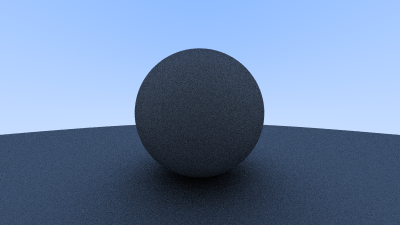
\includegraphics[width=4cm]{slike/img-1.07-first-diffuse.png}
	\end{center}
	\begin{itemize}
		\item Slike je previše tamna
	\end{itemize}
\end{frame}

\begin{frame}{Difuzni materijal, $\gamma$ korekcija}
	\begin{itemize}
		\item \textit{Dijelimo} intenzitet s nekim intenzitetom
		\item Potrebno je napraviti korekciju
		\item Boju \textit{staviti} na potenciju $1/\gamma$
	\end{itemize}
	\begin{center}
		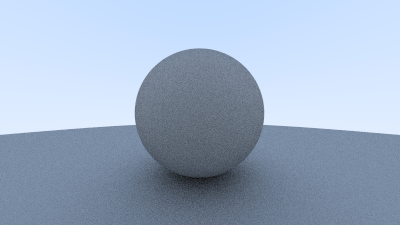
\includegraphics[width=4cm]{slike/img-1.08-gamma-correct.png}
	\end{center}
\end{frame}


\begin{frame}{Refleksija, opet}
	\begin{columns}
		\begin{column}{0.3\textwidth}
			\begin{center}
				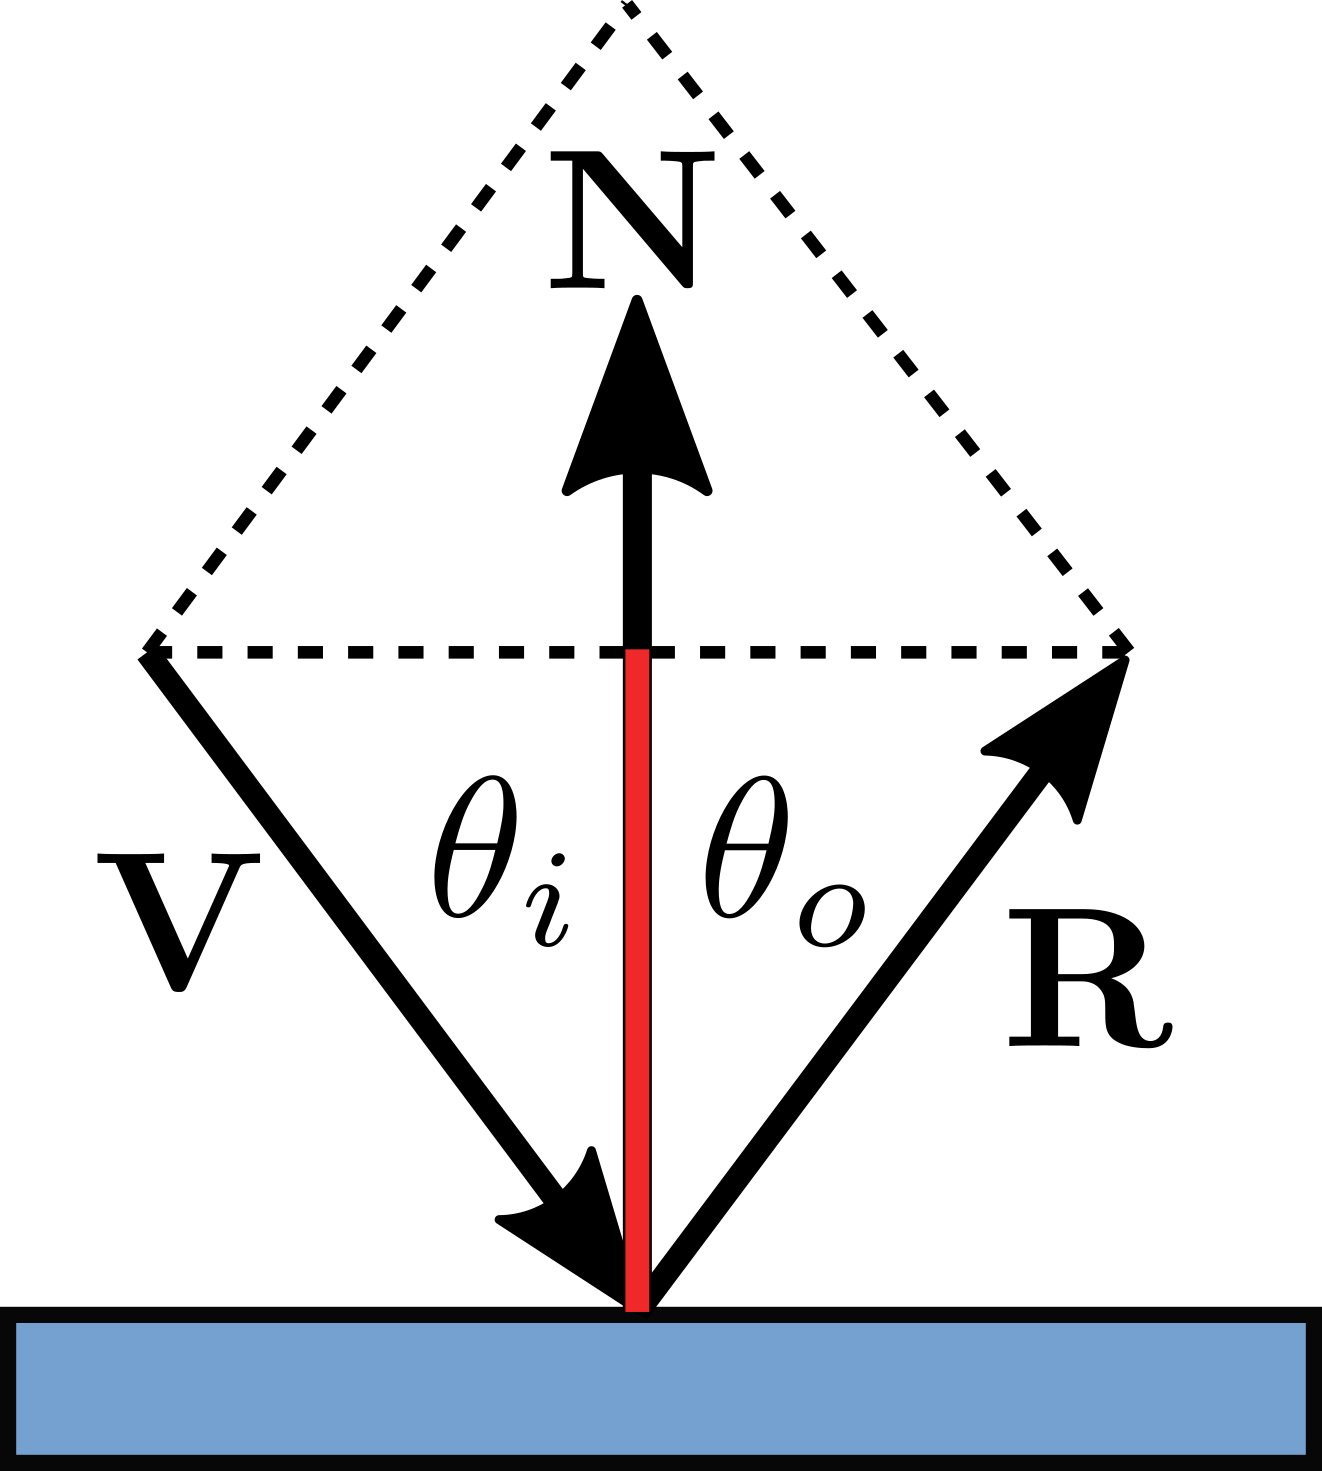
\includegraphics[width=3cm]{slike/refleksija_02.png}
			\end{center}
		\begin{align*}
		\theta= \theta_i = \theta_o
		\end{align*}
		\end{column}
		\begin{column}{0.7\textwidth}
		\begin{align*}
		-\mathbf{V} + \mathbf{R} & = 2 \cos \theta \mathbf{N} = 2(-\mathbf{V} \cdot \mathbf{N})\mathbf{N} \\
		\mathbf{R} & = \mathbf{V} - 2(\mathbf{V} \cdot \mathbf{N})\mathbf{N}
		\end{align*}
		\end{column}
	\end{columns}

Umjesto \textit{nasumične zrake}, odašiljemo samo jednu, u $\mathbf{R}$ smjeru.
\begin{center}
	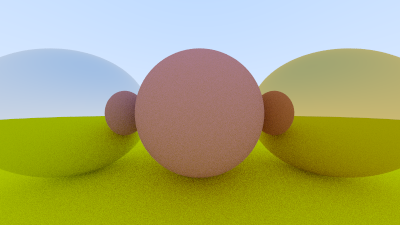
\includegraphics[width=4cm]{slike/img-1.11-metal-shiny.png}
\end{center}
\end{frame}
\begin{frame}{Refleksija, opet}
	\begin{columns}
		\begin{column}{0.3\textwidth}
			\begin{center}
				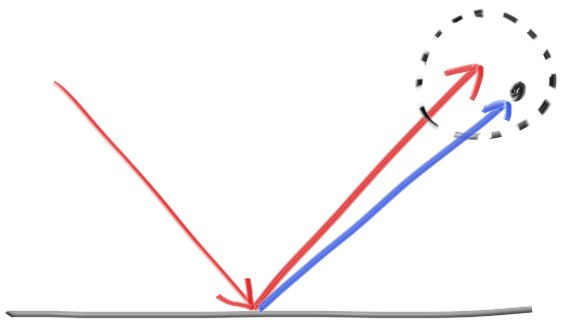
\includegraphics[width=3cm]{slike/fig-1.12-reflect-fuzzy.jpg}
			\end{center}
		\end{column}
		\begin{column}{0.7\textwidth}
			Možda je ipak bolje odašiljati nasumične reflektirane zrake pomoću male sfere. \\
			Što veća sfera, refleksija je mutnija.
		\end{column}
	\end{columns}
	
	\begin{center}
		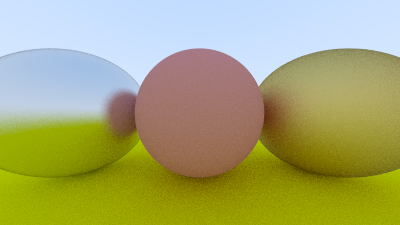
\includegraphics[width=4cm]{slike/img-1.12-metal-fuzz.png}
	\end{center}
\end{frame}


\section{Prozirnost, refrakcija}
\begin{frame}{Prozirnost, refrakcija}

\begin{center}
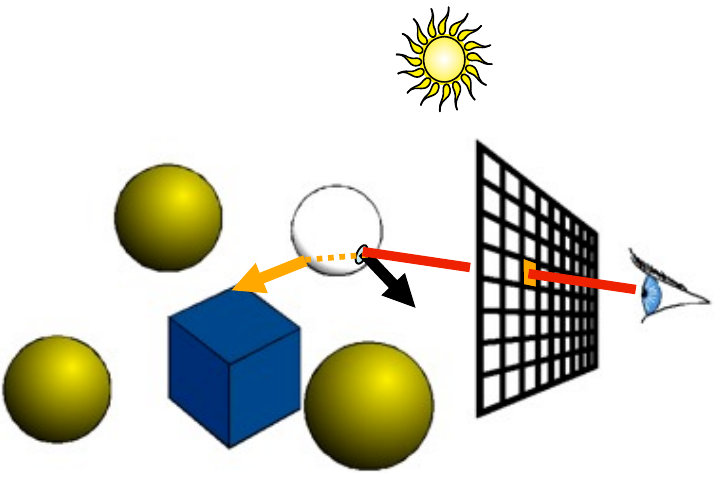
\includegraphics[width=5cm]{slike/prozirnost_01.png}
\end{center}
\begin{itemize}
\item Odaslati zraku u \textit{refrakcijskom} smjeru
\item pomnožiti s koeficijentom refrakcije $k_t$
\end{itemize}

\end{frame}

\begin{frame}{Prozirnost, contd.}

\begin{center}
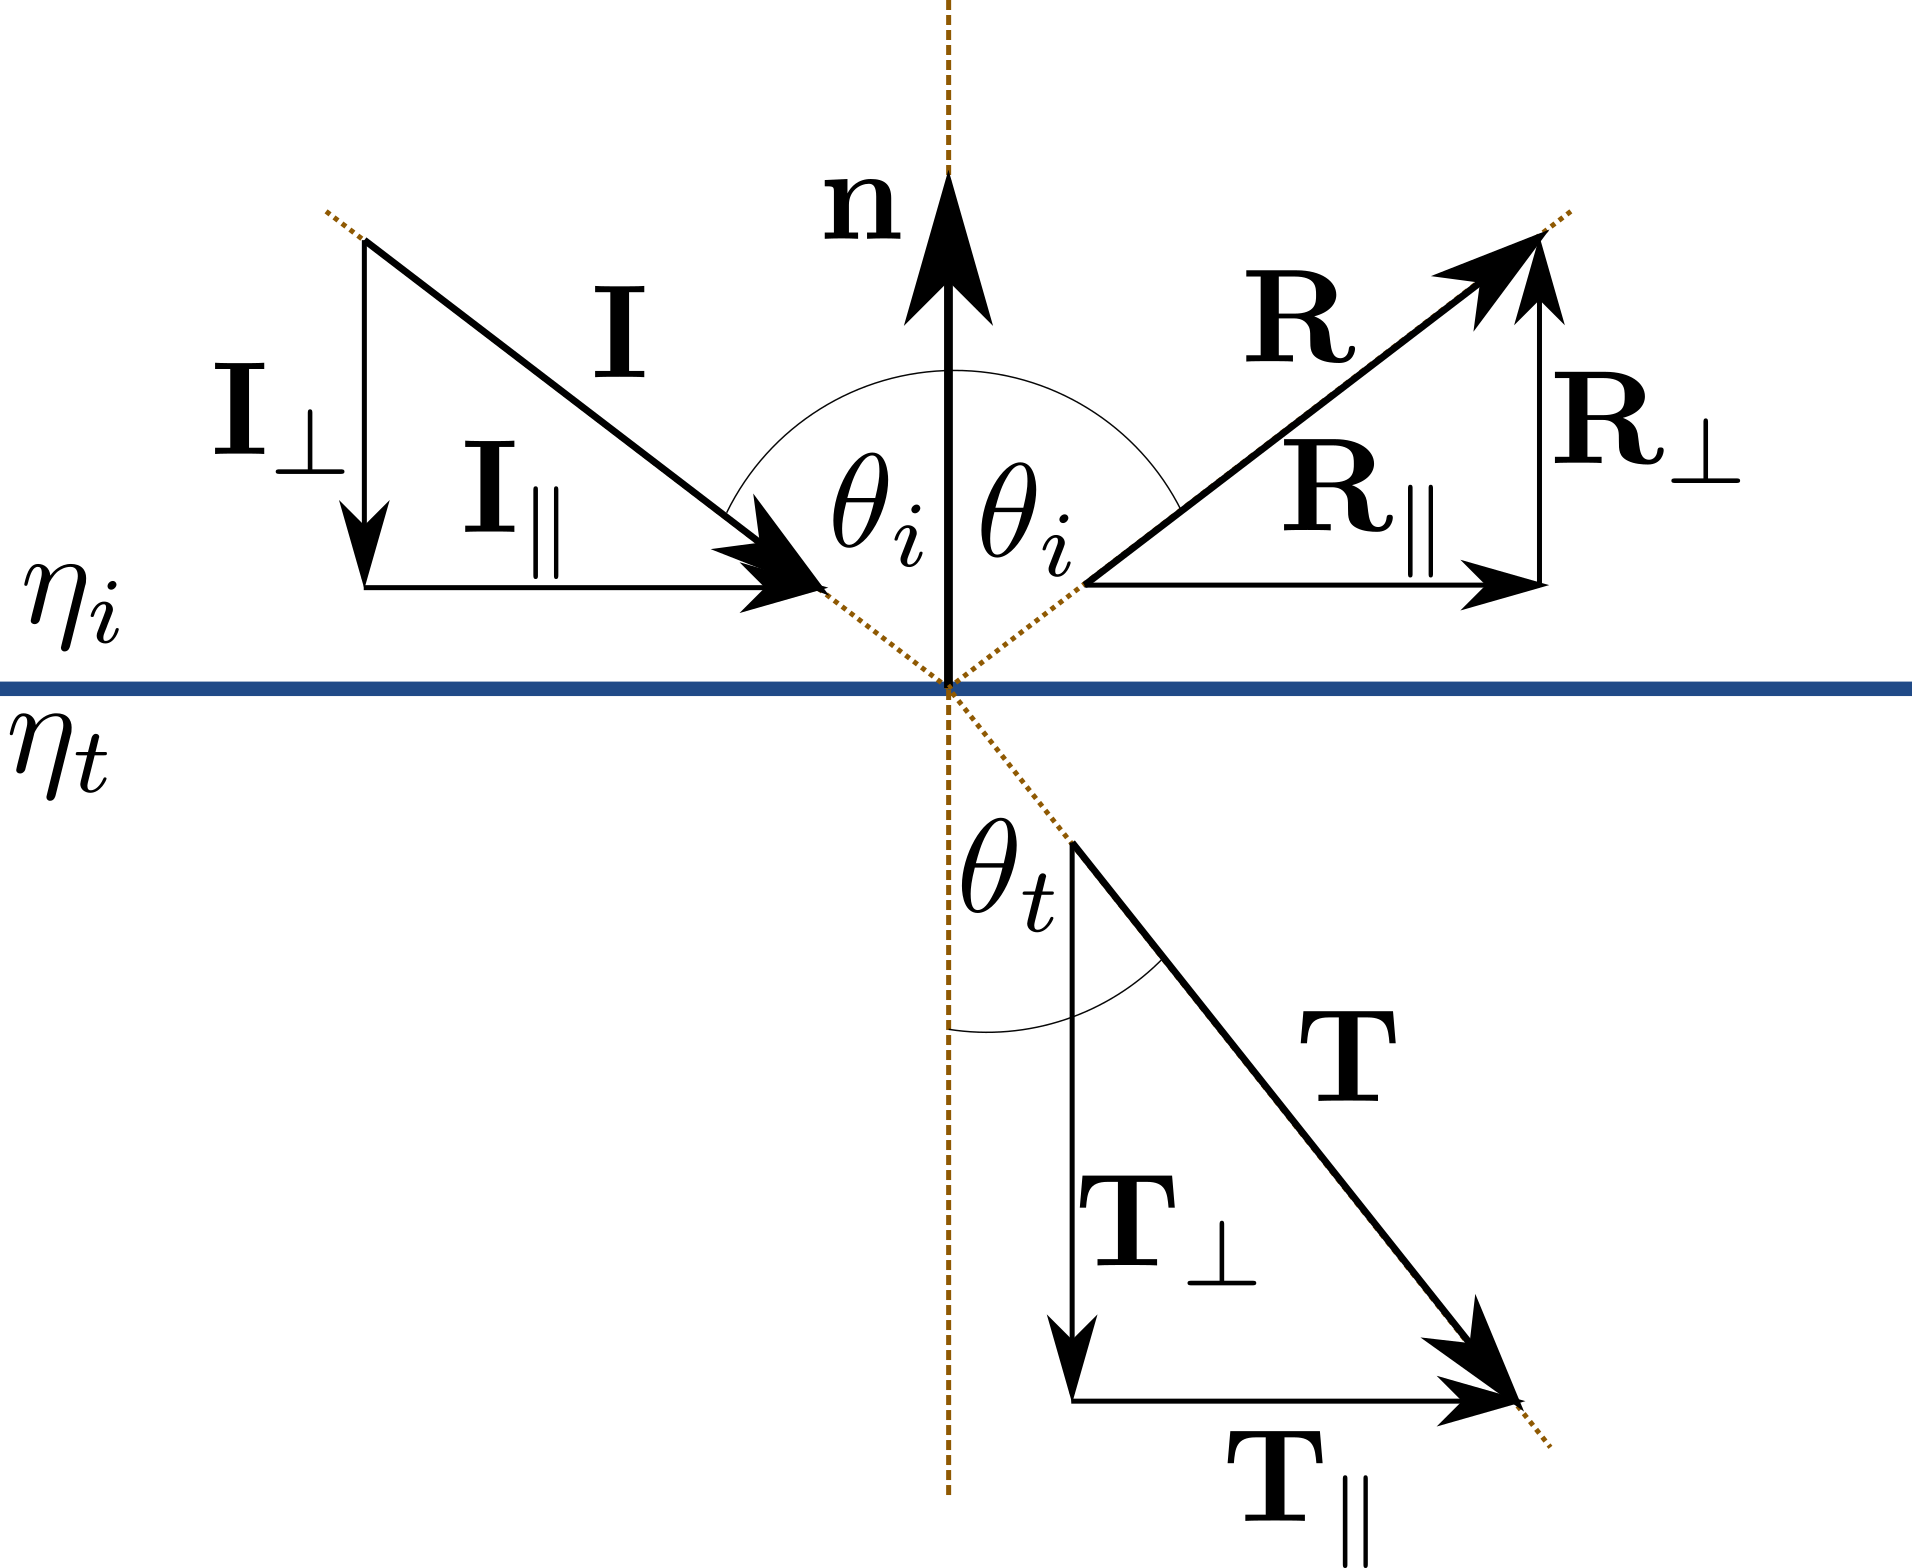
\includegraphics[width=5cm]{slike/prozirnost.png}
\end{center}
\begin{itemize}
\item dva materijala, dva indeksa refrakcije, $\eta_i$ i $\eta_t$
\end{itemize}
\begin{columns}
	\begin{column}{0.5\textwidth}
		Snell-Descartes -ov zakon zakon:
		\begin{align*}
		\sin \eta_i \theta_i = \eta_t \sin\theta_t%  \\
		% \frac{\sin\theta_t}{\sin\theta_i} = \frac{\eta_t}{\eta_i} = \eta_r
		\end{align*}
		% Relativni indeks refrakcije: $\eta_r$\\
		Cilj je odrediti smjer zrake $\mathbf{T}$
	\end{column}
	\begin{column}{0.5\textwidth}
		\begin{center}
			\begin{tabular}{ l r } 
				\textbf{Medij} & $\eta$ \\
				\hline
				Vakuum & $1.0$  \\ 
				Zrak ($0$ m n. m.) & $1.00029$  \\ 
				Voda ($20$ °C) & $1.33$  \\ 
				Staklo & $1.5$-$1.6$  \\ 
				Dijamant & $2.42$  \\ 
				\hline
			\end{tabular}
		\end{center}
	\end{column}
\end{columns}

\end{frame}

\begin{frame}{Prozirnost, kako odrediti $\mathbf{T}$}
\begin{center}
	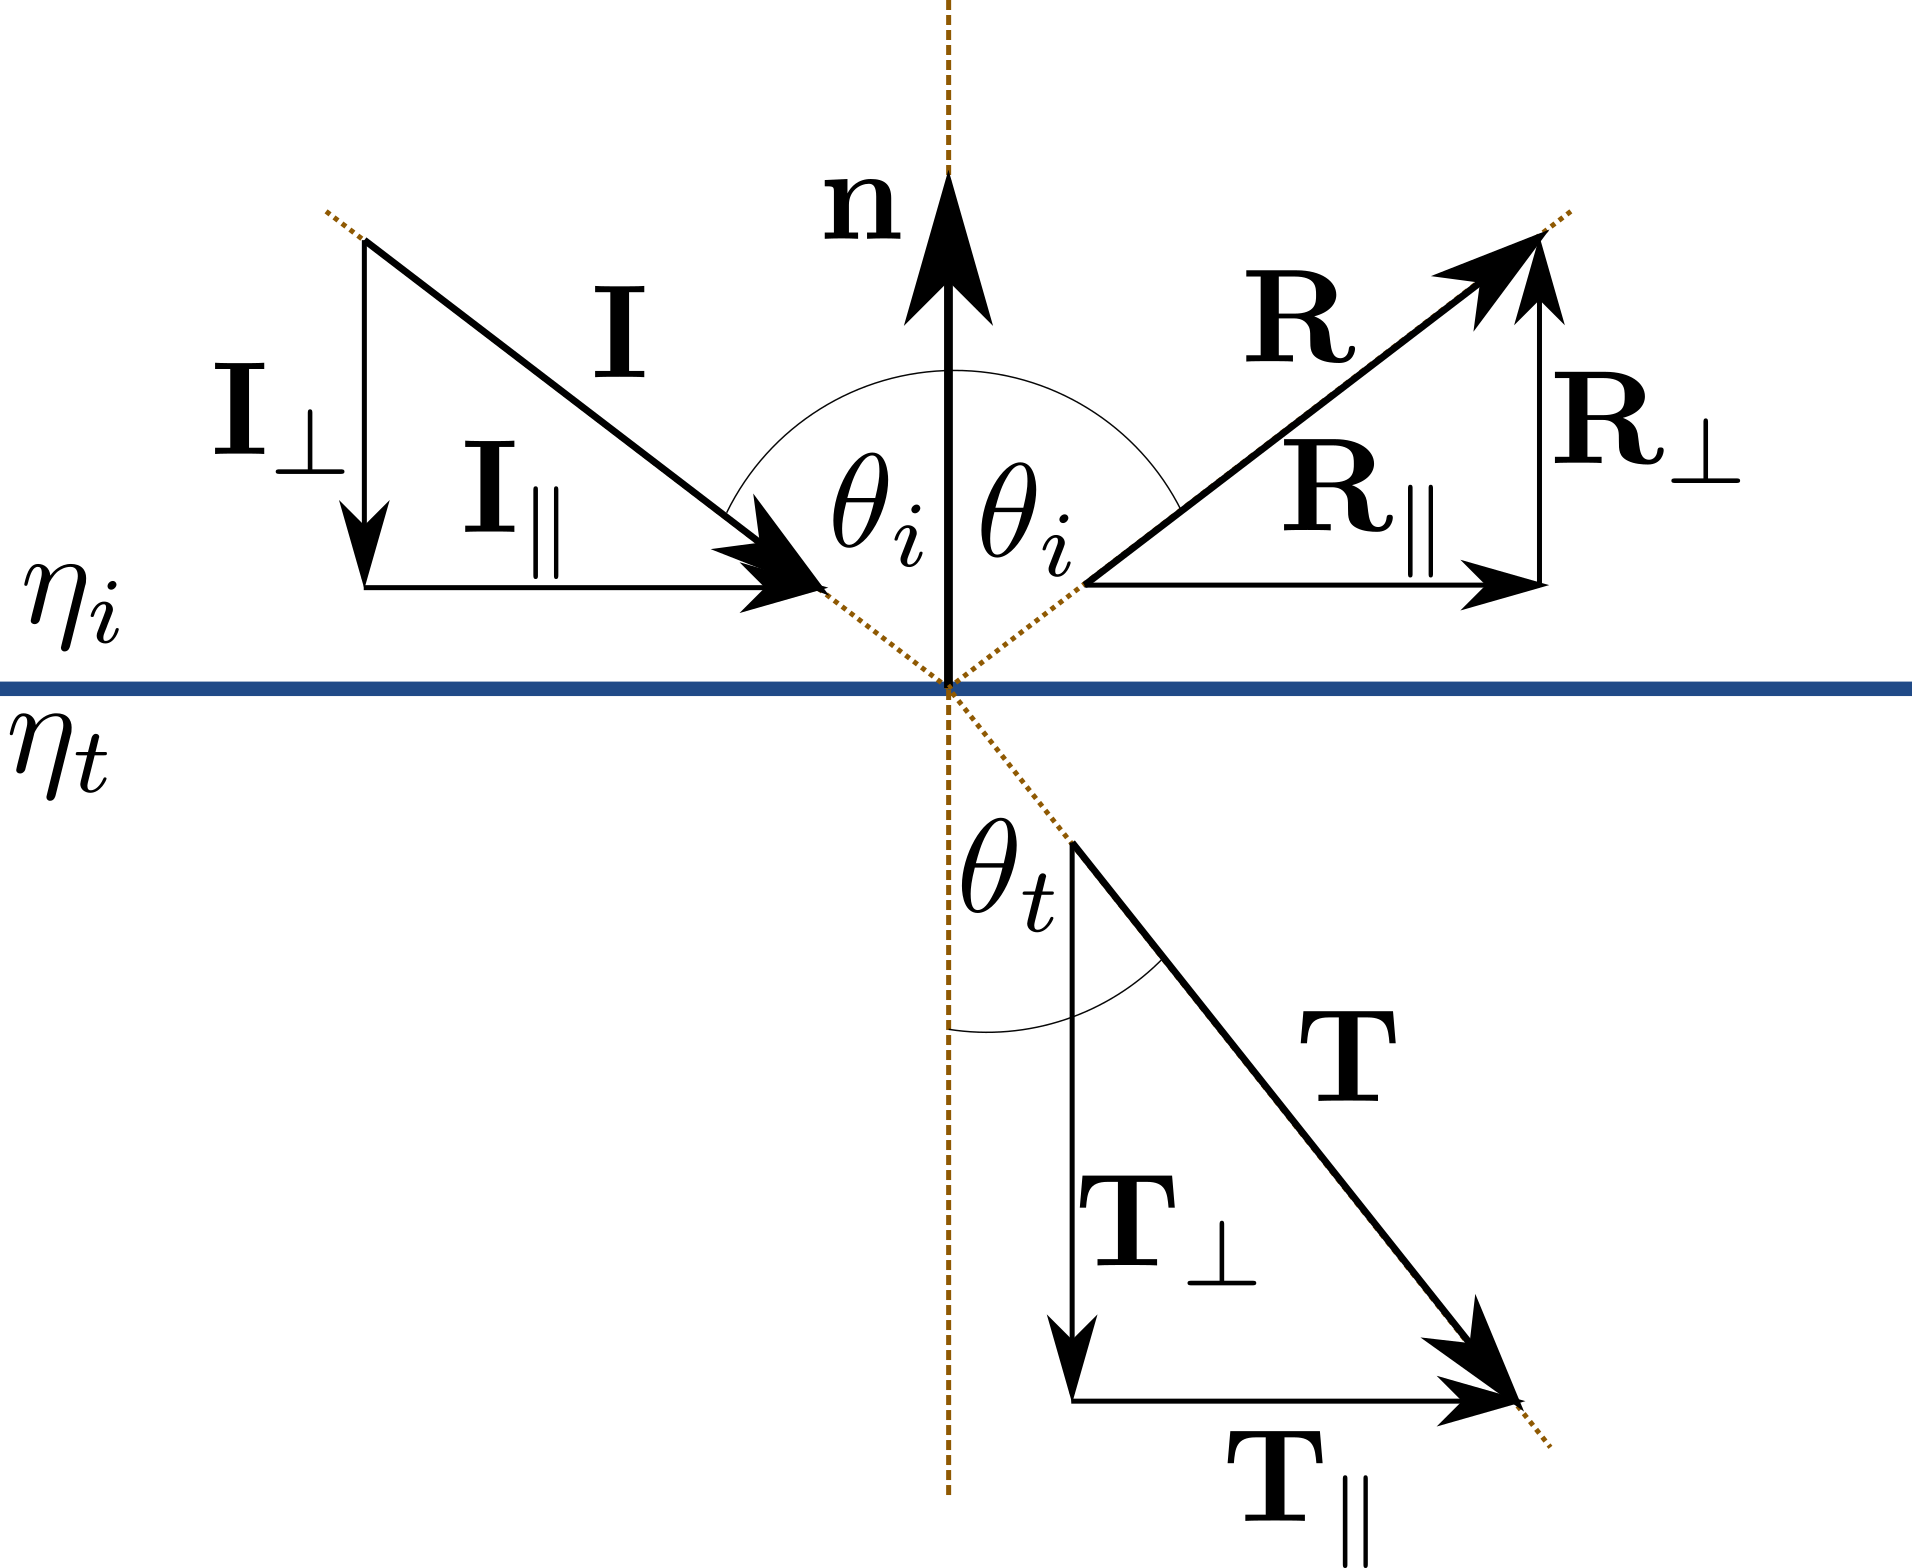
\includegraphics[width=5cm]{slike/prozirnost.png}
\end{center}
\begin{align*}
\mathbf{T} = \mathbf{T}_\parallel + \mathbf{T}_\perp
\end{align*}
\begin{align*}
\mathbf{T}_\parallel = \frac{\eta_i}{\eta_t}\mathbf{I}_\parallel = \frac{\eta_i}{\eta_t}(\mathbf{I} + \cos \theta_i \mathbf{n})
\end{align*}
Sitnica: $ \cos \theta_i = \mathbf{I} \cdot \mathbf{n}$
\begin{align*}
\mathbf{T}_\perp = -\sqrt{1- |\mathbf{T}_\parallel|^2}\mathbf{n}
\end{align*}
\begin{align*}
\mathbf{T} = \mathbf{T}_\parallel + \mathbf{T}_\perp = \frac{\eta_i}{\eta_t}\mathbf{I} + \left(\frac{\eta_i}{\eta_t} \cos \theta_i - \sqrt{1- |\mathbf{T}_\parallel|^2}\right)\mathbf{N}
\end{align*}
%koristiti samo skalarne produkte\ldots
\end{frame}

\begin{frame}{Prozirnost, kako odrediti $\mathbf{T}$, contd.}
	\begin{align*}
	\mathbf{T} & = \frac{\eta_i}{\eta_t}\mathbf{I} + \left(\frac{\eta_i}{\eta_t} \cos \theta_i - \sqrt{1- |\mathbf{T}_\parallel|^2}\right)\mathbf{n} \\
	  & = \frac{\eta_i}{\eta_t}\mathbf{I} + \left(\frac{\eta_i}{\eta_t} \cos \theta_i - \sqrt{1- \sin^2 \theta_t}\right)\mathbf{n}
	\end{align*}
	Par identiteta:
	\begin{itemize}
		\item $ \cos \theta_i = \mathbf{I} \cdot \mathbf{N}$
		\item $\sin^2 \theta_t = (\frac{\eta_i}{\eta_t})^2\sin^2 \theta_i = (\frac{\eta_i}{\eta_t})^2(1-\cos^2 \theta_i)$
	\end{itemize}
\end{frame}

%\begin{frame}{Prozirnost, kako odrediti $\mathbf{T}$, contd.}
%	Ovdje smo stali:
%	\begin{align*}
%	\mathbf{T} = \left(\eta_r\cos\theta_i - \sqrt{1-\eta_r^2\sin^2\theta_i}\right)\mathbf{N} - \eta_r\mathbf{I} 
%	\end{align*}
%	Opet trigonometrija: $\sin^2 \alpha + \cos^2 \alpha= 1$
%	\begin{align*}
%	\mathbf{T} = \left(\eta_r\cos\theta_i - \sqrt{1-\eta_r^2(1-\cos^2\theta_i)}\right)\mathbf{N} - \eta_r\mathbf{I}
%	\end{align*}
%	Konačno, $\mathbf{N}\cdot \mathbf{I}= \cos\theta_i$
%	
%	\begin{block}{Konačan izraz}
%		\begin{align*}
%		\mathbf{T} = \left(\eta_r(\mathbf{N}\cdot \mathbf{I}) - \sqrt{1-\eta_r^2(1-(\mathbf{N}\cdot \mathbf{I})^2)}\right)\mathbf{N} - \eta_r\mathbf{I}
%		\end{align*}
%		Sve što nam treba:
%		\begin{itemize}
%			\item normala
%			\item smjer od kuda dolazi zraka
%			\item koeficijent refrakcije
%		\end{itemize}
%	\end{block}
%\end{frame}

\begin{frame}{Refrakcija i refleksija?}
	\begin{itemize}
		\item Što ako je zraka unutar materijala s većim indeksom refrakcije?
	\end{itemize}
	\begin{align*}
	\eta_i \sin \theta_i = \eta_t \sin \theta_t
	\end{align*}
	\begin{itemize}
		\item Ili:
	\end{itemize}
	\begin{align*}
	\sin \theta_t = \frac{\eta_i}{\eta_t} \sin \theta_i
	\end{align*}
	\begin{itemize}
		\item Ako je $\sin \theta_i > \frac{\eta_t}{\eta_i}$, onda $\sin \theta_t > 1$! 
		\item Potpuna unutrašnja refleksija (\textit{total internal reflection})
	\end{itemize}
	Još jedan uvjet:
	\begin{align*}
		\sin \theta_t = \frac{\eta_i}{\eta_t} \sin \theta_i \Leftrightarrow \sin \theta_i \leq \frac{\eta_t}{\eta_i}
	\end{align*}
\end{frame}

\begin{frame}{Kritični kut}
	Iz \begin{align*}
	\mathbf{T} = \frac{\eta_i}{\eta_t}\mathbf{I} + \left(\frac{\eta_i}{\eta_t} \cos \theta_i - \sqrt{1- \sin^2 \theta_t}\right)\mathbf{n}
	\end{align*}
	mora vrijediti $\sin^2 \theta_t < 1$, odnosno, vrijedi uvjet $\sin \theta_i \leq \frac{\eta_t}{\eta_i}$.
	
	\begin{block}{}
		Ako uvjet $\sin \theta_i \leq \frac{\eta_t}{\eta_i}$ \alert{nije} zadovoljen, onda nema \alert{refrakcije}.
		
		Ulazni kut pri kojem taj uvjet prestaje vrijediti: 
		\begin{align*}
			\theta_c = \arcsin \frac{\eta_t}{\eta_i} \Leftrightarrow \eta_i > \eta_t
		\end{align*}
	\end{block}
\end{frame}

\begin{frame}{Potpuna unutrašnja refleksija}
	\begin{block}{story time!}
		Svaki foton koji nailazi na \textit{granicu} u smjeru $\mathbf{I}$ može:
		\begin{itemize}
			\item proći kroz granicu u smjeru $\mathbf{T}$ (transmisija)
			\item odbiti se u smjeru  $\mathbf{R}$ (refleksija)
		\end{itemize}
		Od svih fotona koji naiđu na granicu, dio se reflektira(\textit{reflectance}, $R$) a dio se \textit{produži dalje} (\textit{transmittance}, $T$). Odnosno,
		$$T + R = I$$
		Količina reflektiranih i transmisijskih fotona ovisi o refrakcijskim indeksima $\eta_i$ i $\eta_t$, kao i o kutu
		upada $\theta_i$, što je opisano \textit{Fresnelovim} jednadžbama.
	\end{block}
	\begin{block}{tldr}
		Fresnelove jednadžbe previše komplicirane, potrebno smisliti način kako modelirati prozirnost i refleksiju.
		
		Npr. staklo ili voda su prozirni, ali u nekim uvjetima mogu poslužiti kao ogledalo.
	\end{block}
\end{frame}

\begin{frame}{Schlickova aproksimacija}
	Aproksimacija \textit{Fresnelovih} jednadžbi:
	\begin{align*}
	\mathbf{R}_{Schlick}(\theta_i) = R_0 + (1-R_0)(1-\cos \theta_i)^5
	\end{align*}
	gdje je 
	$$
	R_0 = \left(\frac{\eta_i-\eta_t}{\eta_i+\eta_t}\right)^2
	$$
	Gornji izraz ne modelira refleksiju za $\eta_i > \eta_t$. Potrebno koristiti $\cos \theta_t$ umjesto $\cos \theta_i$ za prethodni uvjet:
	\begin{align*}
	\mathbf{R}_{Schlick}(\theta_i) \begin{cases}
		R_0 + (1-R_0)(1-\cos \theta_i)^5 & \eta_i\leq\eta_t \\
		R_0 + (1-R_0)(1-\cos \theta_t)^5 & \eta_i > \eta_t \land \neg \mathrm{TIR}\\
		1 & \land \mathrm{TIR}
	\end{cases}      
	\end{align*}
\end{frame}

\section{Fokus}
\begin{frame}{Focus blur}
	\begin{center}
		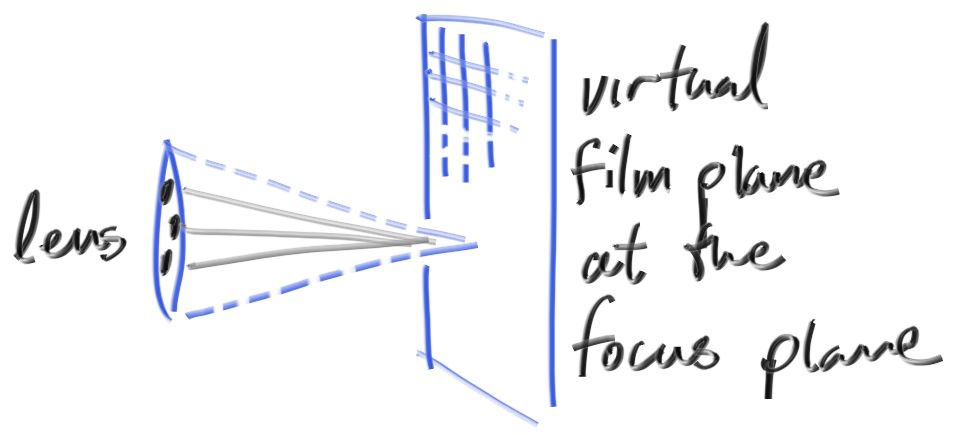
\includegraphics[width=5cm]{slike/fig-1.18-cam-film-plane.jpg}
	\end{center}
\begin{itemize}
	\item Blur: generirati zrake koje se odašilju unutar diska čiji je centar točka gledišta.
	\item Fokus svugdje: sve se zrake odašilju iz jedne točke, ili, disk polumjera $0$
\end{itemize}

	\begin{center}
		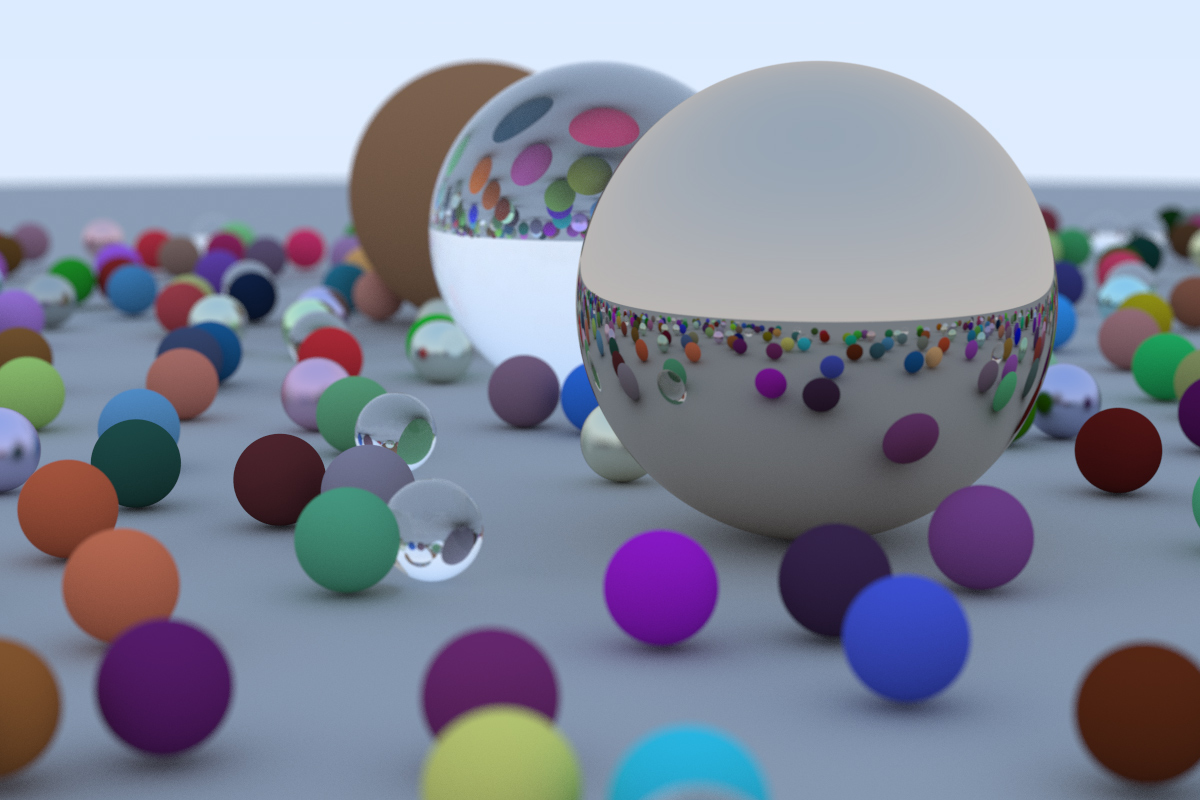
\includegraphics[width=5cm]{slike/img-1.21-book1-final.jpg}
	\end{center}
\end{frame}

\section{Teksture, opet}
\begin{frame}{Teksture i sfere}
	\begin{itemize}
		\item Za sferu $r=1$:
		\item Tekstura: $0 \leq u,v \leq 1$
		\item Sferne koordinate: $(\theta, \phi)$, $\theta$
		\begin{itemize}
			\item analogija: geografska dužina $\theta$ i širina $\phi$
		\end{itemize}
		\item Preslikavanje: $u = \phi/(2 \pi)$, $v = \theta / \pi$
		\item Iz: $x = -\cos \theta$, $y = -\cos (\phi) \sin (\theta)$, $z = \sin (\phi) \cos (\theta)$
		\item $\phi = \text{atan2}(-z, x) + \pi$, $\theta= \arccos(-y)$
		\begin{itemize}
			\item $\text{atan2}$ je $\tan$, ali...
			\item za interval $-\pi < \text{atan2(y,x)} \leq \pi$
			\item Ovdje je $x = \cos(\alpha)$, $y = \sin (\alpha)$
		\end{itemize}
	\end{itemize}
\end{frame}

\begin{frame}{Generiranje teksture}
	Ovo je jednostavno:
	\begin{columns}
		\begin{column}{0.5\textwidth}
			\begin{itemize}
				\item Uzmimo koordinatu točke ($x_p$)
				\item $c =\sin (x_p)$
				\item $c >0$, jedna boja
				\item $c <0$, druga boja
				\item želimo li kontrolirati širinu $w$: $c =\sin (\pi x_p / w)$
				\item Želimo li interpolirati boje: 
				\begin{itemize}
					\item $t = (1 + \sin (\pi x_p / w))/2$
					\item $(1-t)c_0 + t c_1$ - linearna interpolacija
				\end{itemize}
			\end{itemize}
		\end{column}
		\begin{column}{0.5\textwidth}
			\begin{center}
				
\includegraphics[width=2cm]{slike/stripes_teksture.png}
			\end{center}
		\end{column}
	\end{columns}
\end{frame}

\begin{frame}{Perlin noise}
	\begin{itemize}
		\item Umjesto regularne strukure, želimo nasumičnu, pjegavu, išaranu teksturu
		\item Kreirati \textit{random} broj za svaku točku nije baš pametno 
		\item Želimo glatku strukturu, bez odricanja nasumične komponente
	\end{itemize}
	
	
%	\begin{align*}
%		n(x, y, z) = \sum_{i = \lfloor x \rfloor}^{\lfloor x \rfloor + 1}
%		\sum_{j = \lfloor y \rfloor}^{\lfloor y \rfloor + 1}
%		\sum_{k = \lfloor z \rfloor}^{\lfloor z \rfloor + 1}
%		\Omega_{ijk}(x-i,y-j, z-k)
%	\end{align*}
%	
%	\begin{align*}
%	\Omega_{ijk}(u, v, w) = \omega(u)\omega(v)\omega(w)(\Gamma\cdot())
%	\end{align*}
\end{frame}
\begin{frame}{Perlin noise}
	Za svaku točku  teksture $x, y$ kreiramo jedinični kvadrat $\left[x, y \right] \% 1$
	\begin{center}
		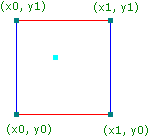
\includegraphics[width=2cm]{slike/logic01.png}
	\end{center}
	Za sve točke kreiramo \textit{pseudo random} vektor
	\begin{center}
		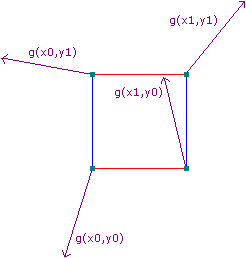
\includegraphics[width=3cm]{slike/logic02.png}
	\end{center}
\end{frame}

\begin{frame}{Perlin noise}
	Izračunamo vektore od točaka kvadrata do točke $x, y$ (\textit{distance} vektor)
	\begin{center}
		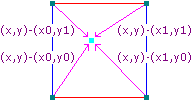
\includegraphics[width=2cm]{slike/logic03.png}
	\end{center}
	\begin{itemize}
		\item Sada za svaku točku kvadrata izračunamo skalarni produkt \textit{gradient} i \textit{distance} vektora.
		\item Rezultat? Skalarni produkt je pozitivan u smjeru gradijenta, negativan inače
		\item Slika prikazuje utjecaj pozitivnih i negativnih skalarnih produkata
	\end{itemize}
	\begin{center}
		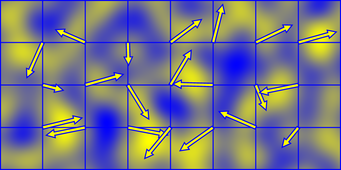
\includegraphics[width=3cm]{slike/logic04.png}
	\end{center}
\end{frame}

\begin{frame}{Perlin noise}
	\begin{itemize}
		\item potrebno interpolirati ta 4 skalarna produkta, koristeći tzv. \textit{weight function}.
		\item \textit{weight function} primjer: $w(t) = 2|t|^3 - 3|t|^2 + 1$
	\end{itemize}
	
	\begin{itemize}
		\item Ključno: Perlin noise se ponavlja
		\item Za svaku 3D točku uvijek vraća isti nasumični broj.
		\item Bliske točke vraćaju slične brojeve
	\end{itemize}
\end{frame}

\begin{frame}{Perlin noise, stvarno kraj}
	\begin{align*}
		perlin(x, y) = \sum_{k}noise(freq(k)\cdot (x,y))\cdot scale(k)
	\end{align*}
	\begin{align*}
	freq(k) = 2^k 
	\end{align*}
\end{frame}
%\begin{frame}{Prozirnost, kako odrediti $\mathbf{T}$, contd.}
%\begin{align}
%\mathbf{T} &= -\mathbf{N}\cos\theta_t + \mathbf{M}\sin\theta_t \\
%&= -\mathbf{N}\cos\theta_t + ((\mathbf{N}\cos\theta_i - \mathbf{I})/\sin\theta_i)\sin\theta_t \\
%&= -\mathbf{N}\cos\theta_t + (\mathbf{N}\cos\theta_i - \mathbf{I})\eta_r \\
%&= \left(\eta_r\cos\theta_i - \cos\theta_t\right)\mathbf{N} - \eta_r\mathbf{I} \\
%&= \left(\eta_r\cos\theta_i - \sqrt{1-\sin^2\theta_t}\right)\mathbf{N} - \eta_r\mathbf{I} \\
%&= \left(\eta_r\cos\theta_i - \sqrt{1-\eta_r^2\sin^2\theta_i}\right)\mathbf{N} - \eta_r\mathbf{I} \\
%&= \left(\eta_r\cos\theta_i - \sqrt{1-\eta_r^2(1-\cos^2\theta_i)}\right)\mathbf{N} - \eta_r\mathbf{I} \\
%\mathbf{T} &= \left(\eta_r(\mathbf{N}\cdot \mathbf{I}) - \sqrt{1-\eta_r^2(1-(\mathbf{N}\cdot \mathbf{I})^2)}\right)\mathbf{N} - \eta_r\mathbf{I}
%\end{align}
%\end{frame}
%
%\begin{frame}{Prozirnost, kako odrediti $\mathbf{T}$, contd.}
%\begin{center}
%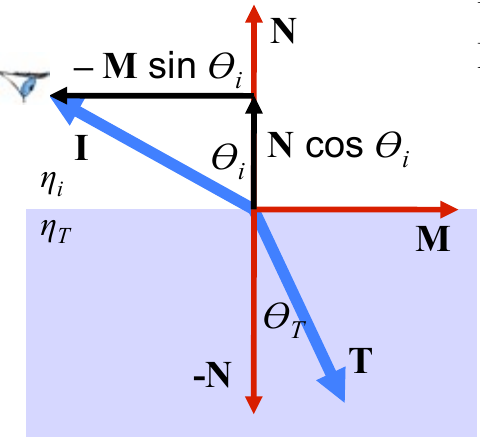
\includegraphics[width=3cm]{slike/prozirnost_03.png}
%\end{center}
%\begin{itemize}
%\item  U izvodu smo prvo zamijenili $\mathbf{M}$ iz $\mathbf{M} = (\mathbf{N}\cos\theta_i - \mathbf{I})/\sin\theta_i$
%\item uveli koeficijent refrakcije $\eta_r$
%\item Iskoristili $\sin^2 \alpha + \cos^2 \alpha= 1$
%\item Izrazili $\sin \theta_t$ pomoću $\sin \theta_i$
%\item Na kraju iskoristili činjenicu da je $\mathbf{N}\cdot \mathbf{I}= \cos\theta_i$
%\end{itemize}
%
%\end{frame}
\plain{Pitanja?}
\end{document}